\question{}

You now train your transformer on a cluster. The cluster's interconnect is
wired as a \emph{binary tree}: the $8$ \textbf{leaves} are the compute nodes
$C_0,\dots,C_7$ and every \textbf{internal node} is a router. Each router has at
$4$ available ports. Each non-root router uses one port towards its parent and one towards
each of its two children, leaving one unused.
We assume that all links and ports have the same bandwidth.

\begin{center}
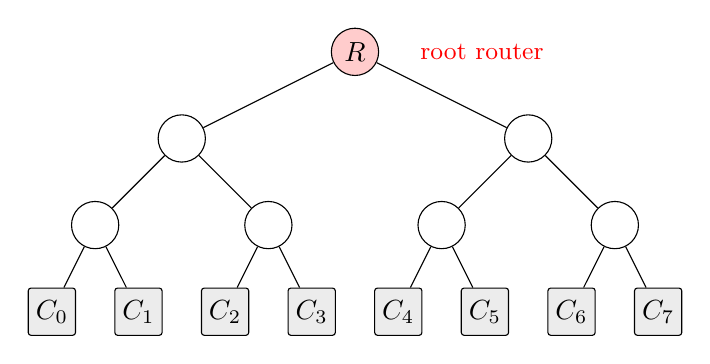
\begin{tikzpicture}[
  level distance=11mm,
  level 1/.style={sibling distance=44mm},
  level 2/.style={sibling distance=22mm},
  level 3/.style={sibling distance=11mm},
  router/.style={circle,draw,minimum size=6mm,inner sep=0pt},
  cnode/.style={draw,rounded corners=1pt,minimum size=6mm,inner sep=1pt,fill=gray!15},
  edge from parent/.style={draw,-}]
\node[router,fill=red!20] (root) {$R$}
  child {node[router]{}
    child {node[router]{} child{node[cnode]{$C_0$}} child{node[cnode]{$C_1$}}}
    child {node[router]{} child{node[cnode]{$C_2$}} child{node[cnode]{$C_3$}}}}
  child {node[router]{}
    child {node[router]{} child{node[cnode]{$C_4$}} child{node[cnode]{$C_5$}}}
    child {node[router]{} child{node[cnode]{$C_6$}} child{node[cnode]{$C_7$}}}};
\node[red,anchor=west] at ([xshift=4mm]root.east) {\small root router};
\end{tikzpicture}
\end{center}

\begin{parts}
\part Computing the attention scores $R = QK^\top$ in a distributed way requires,
at one point, a \emph{transpose} of a matrix that is spread across the $8$ compute
nodes: each node initially holds a block of rows and, after the transpose, must hold
a block of columns, so every node sends a piece of its data to every other node. You
time this exchange and it is far slower than the individual link speeds would lead
you to expect. Analyse how this collective behaves on the tree interconnect: what
limits its running time, and how does that limit change if the cluster keeps growing as a binary tree?
Justify your answer.
\SetTotalwidth
    \begin{solutionbox}{11cm}
    \textbf{The root router $R$ is the bottleneck.} In a binary tree the only path
    between a left-half leaf and a right-half leaf goes up to the root and back down:
    every left$\leftrightarrow$right message must traverse $R$ and its two links. So
    the whole all-to-all between the halves is funnelled through a single router.

    The \emph{bisection bandwidth} of the tree is just the capacity of those root
    links (a cut separating the left half from the right half severs only the root's
    two links), i.e.\ $O(1)$ regardless of $N$. The left/right exchange moves
    $\Theta(N^2)$ blocks but only $O(1)$ can cross per unit time, so the time grows
    with $N$. Adding compute nodes makes the problem \emph{worse}: more leaves means
    more traffic squeezed through the same root, while the root's throughput stays
    fixed. The bottleneck is the topology, not the number of nodes.
    \end{solutionbox}
\part The company buys \textbf{$5$ more routers} (same $4$-port routers), so you now
have $7 + 5 = 12$ routers in total.
Explain how to use these 5 new routers to improve the running time of the transpose operation.
\SetTotalwidth
    \begin{solutionbox}{20cm}
    This is \emph{exactly} the number
    needed to rewire the cluster as a \emph{butterfly} network connecting the $8$ compute
    nodes.
    A butterfly on $N=2^3=8$ terminals has
    $\log_2 N = 3$ \emph{stages}, each made of $N/2 = 4$ radix-$2$ switches
    ($2$ inputs $+\,2$ outputs $=4$ ports — exactly our routers). That is
    $3\times 4 = 12$ switches, vs.\ the $N-1 = 7$ routers of the tree, hence the
    $12-7 = 5$ extra ones.

    \textbf{Placement.} Arrange the $12$ routers as $3$ columns of $4$. Each compute
    node feeds into a first-stage switch; between consecutive stages, pair the rows
    that differ in one address bit — stride $4$ at stage~1, stride $2$ at stage~2,
    stride $1$ at stage~3 (the perfect-shuffle / FFT wiring). Each pair forms one
    $2\times2$ switch, so every router uses all $4$ ports.

    \begin{center}
    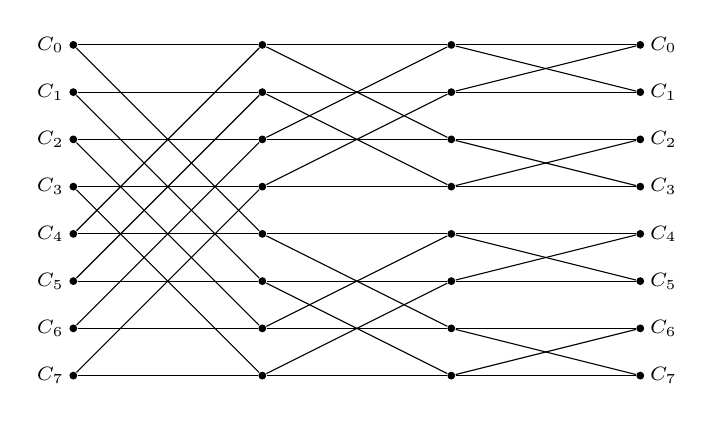
\begin{tikzpicture}[x=12mm,y=-6mm,dot/.style={circle,fill,inner sep=1pt}]
      \foreach \c in {0,1,2,3}
        \foreach \i in {0,...,7}
          \node[dot] (n\c-\i) at (2*\c,\i) {};
      \foreach \i in {0,...,7}{
        \node[left]  at (n0-\i) {\scriptsize $C_\i$};
        \node[right] at (n3-\i) {\scriptsize $C_\i$};
      }
      \foreach \a/\b in {0/4,1/5,2/6,3/7}{
        \draw (n0-\a)--(n1-\a); \draw (n0-\b)--(n1-\b);
        \draw (n0-\a)--(n1-\b); \draw (n0-\b)--(n1-\a);}
      \foreach \a/\b in {0/2,1/3,4/6,5/7}{
        \draw (n1-\a)--(n2-\a); \draw (n1-\b)--(n2-\b);
        \draw (n1-\a)--(n2-\b); \draw (n1-\b)--(n2-\a);}
      \foreach \a/\b in {0/1,2/3,4/5,6/7}{
        \draw (n2-\a)--(n3-\a); \draw (n2-\b)--(n3-\b);
        \draw (n2-\a)--(n3-\b); \draw (n2-\b)--(n3-\a);}
    \end{tikzpicture}
    \end{center}

    \textbf{Why it removes the bottleneck.} The butterfly has bisection width $N/2 = 4$:
    a left/right cut now crosses $4$ links instead of the tree's $2$ at the single
    root, and there is no single shared router any path is forced through. The
    half-to-half all-to-all can use $N/2$ disjoint paths in parallel, so the
    bandwidth scales with the machine instead of being pinned to one root router
    (still with a uniform $\log_2 N = 3$ hops between any two nodes).
    \end{solutionbox}
\end{parts}
